\documentclass[12pt]{article}
\usepackage{tikz}
\usepackage{verbatim}
\usepackage{amsmath,amscd}
\usepackage{graphicx}
\usepackage{amssymb}
\usepackage{epstopdf}
\usepackage{fge}
\usepackage{holtpolt}
\usepackage{mathabx}
%%%%%%%%%%%%%%%%%%%%%%%%%%%%%%
\begin{comment}
...nearshore wave model courtesy of the SWAN group 
\end{comment}
%%%%%%%%%%%%%%%%%%%%%%%%%%%%%
\usetikzlibrary{positioning}
\begin{document}
\pagestyle{empty}
%%%%%%%%%%%%%%%%%%%%%%%%%%%%%
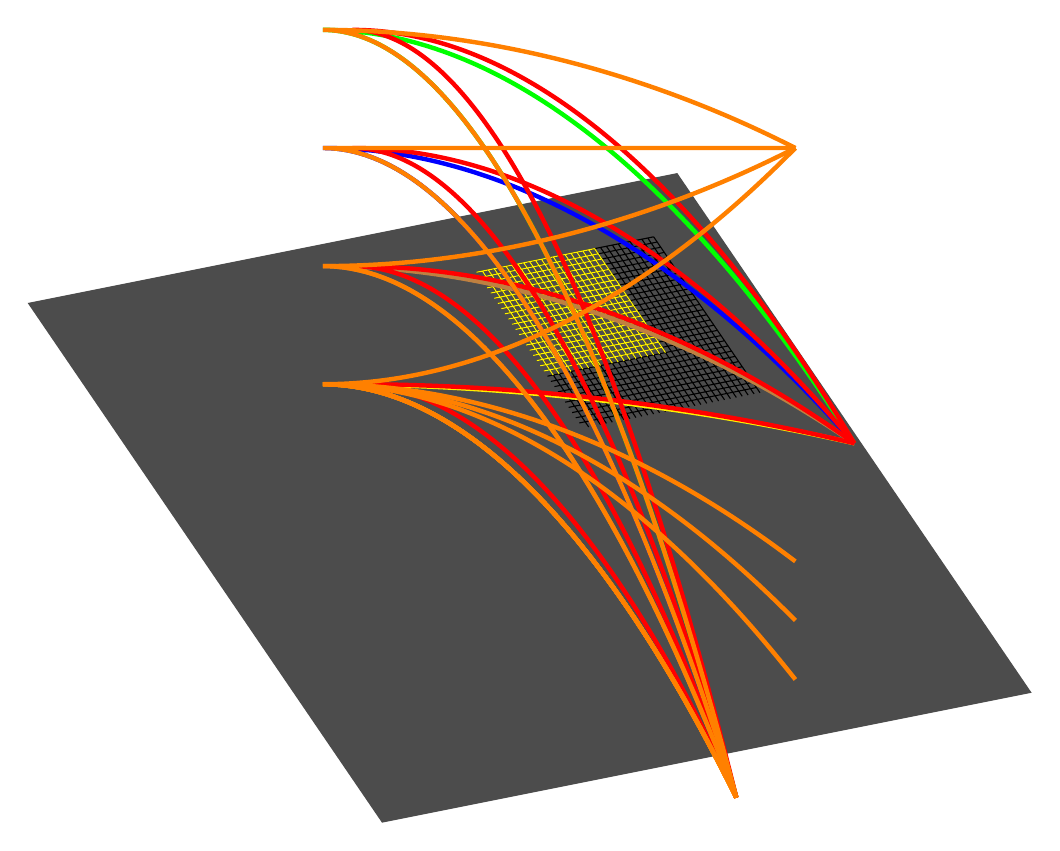
\begin{tikzpicture}[scale=0.75,every node/.style={minimum size=1cm},on grid]
\begin{scope}[
    	yshift=5,every node/.append style={
    	yslant=0.5,xslant=-1},yslant=0.2,xslant=-.6
    	             ]
    	\fill[black,fill opacity=.7] (-6,-5) rectangle (5,5);
    	\draw[step=1mm, black] (1,1) grid (4,4);
	\draw[step=1mm, yellow] (1,2) grid (3,4);%%%%%%BLUE GRID
    	%\draw[green,very thick] (1,1) grid (5,6);
    	%\draw[orange] (0,0) rectangle (5,5);
    \end{scope}
 
 \draw [brown,ultra thick](3,-5) parabola bend (-4,4) (5,1)  ;
\draw [yellow,ultra thick](3,-5) parabola bend (-4,2) (5,1)  ;
\draw [green,ultra thick](3,-5) parabola bend (-4,8) (5,1) ;
\draw [blue,ultra thick](3,-5) parabola bend (-4,6) (5,1)  ;
%\draw [red,ultra thick](3,-5) parabola bend (4,6) (5,1)  ;
\draw [red,ultra thick](3,-5) parabola bend (-3.5,6) (5,1)  ;
\draw [red,ultra thick](3,-5) parabola bend (-3.5,4) (5,1)  ;
\draw [red,ultra thick](3,-5) parabola bend (-3.5,8) (5,1)  ;
\draw [red,ultra thick](3,-5) parabola bend (-3.5,2) (5,1)  ;
\draw [orange,ultra thick](3,-5) parabola bend (-4,2) (4,6)   ;
\draw [orange,ultra thick](3,-5) parabola bend (-4,4) (4,6)   ;
\draw [orange,ultra thick](3,-5) parabola bend (-4,6) (4,6)   ;
\draw [orange,ultra thick](3,-5) parabola bend (-4,8) (4,6)   ;
\draw [orange,ultra thick](3,-5) parabola bend (-4,2) (4,-1)   ;
\draw [orange,ultra thick](3,-5) parabola bend (-4,2) (4,-2)   ;
\draw [orange,ultra thick](3,-5) parabola bend (-4,2) (4,-3)   ;
       \end{tikzpicture}
    
\begin{tikzpicture}[tqft/cobordism/.style={draw}]
\ pi c [ t q f t / pa i r o f pants , name=a ] ;
\ pi c [ t q f t / c y l i n d e r to next , anchor=incoming boundary
1 ,name=c , at=(a−outgoing boundary 1) ] ;
\ pi c [ t q f t / r e v e r s e pa i r o f pants , anchor=incoming
boundary 1 , at=(a−outgoing boundary 2) ] ;
\end{tikzpicture}

 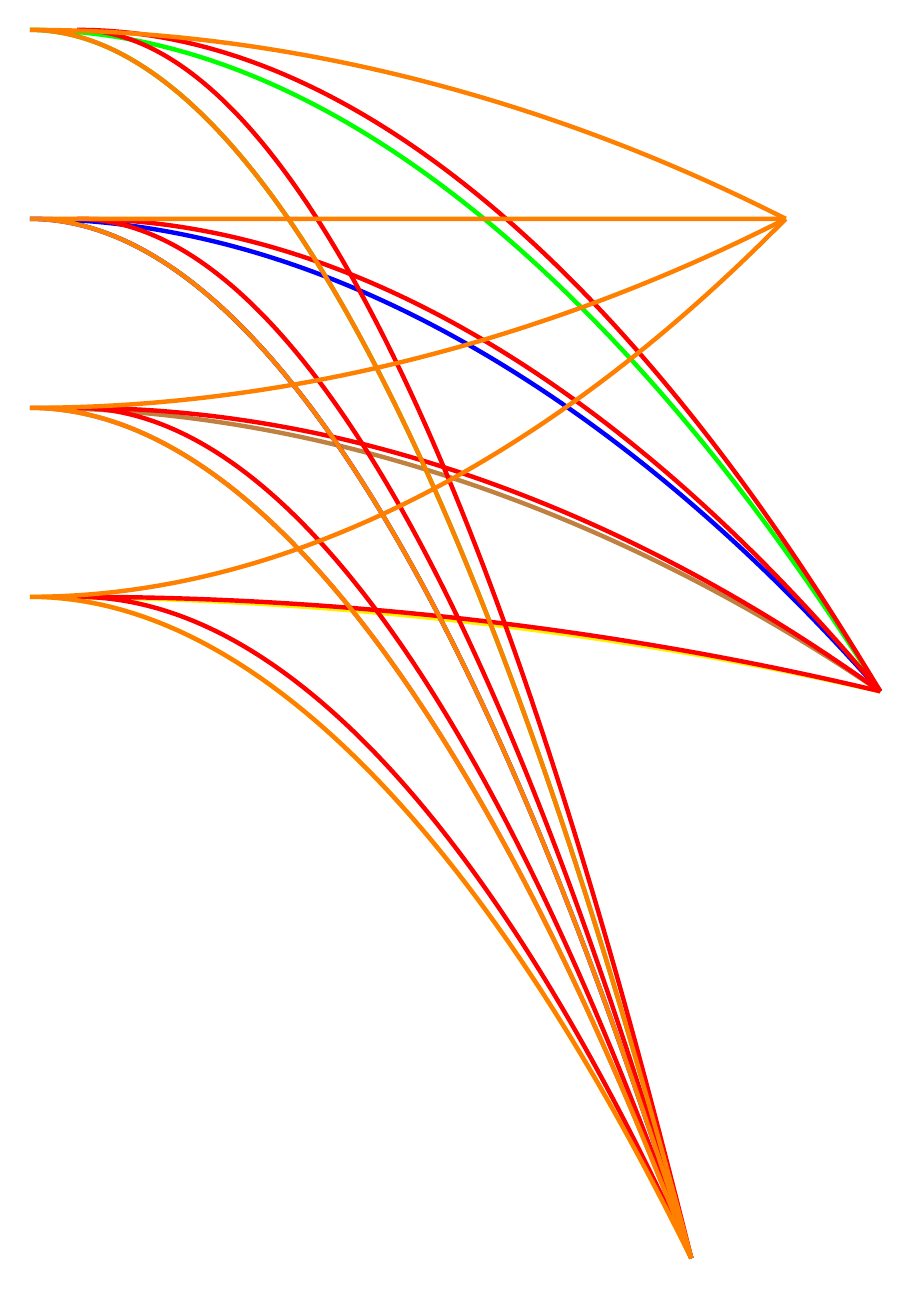
\begin{tikzpicture}[scale=1.2,every node/.style={minimum size=1cm},on grid]
 %\draw [ultra thick](-3,-5) parabola bend (4,4) (5,-1)  ;
\draw [brown,ultra thick](3,-5) parabola bend (-4,4) (5,1)  ;
\draw [yellow,ultra thick](3,-5) parabola bend (-4,2) (5,1)  ;
\draw [green,ultra thick](3,-5) parabola bend (-4,8) (5,1) ;
\draw [blue,ultra thick](3,-5) parabola bend (-4,6) (5,1)  ;
%\draw [red,ultra thick](3,-5) parabola bend (4,6) (5,1)  ;
\draw [red,ultra thick](3,-5) parabola bend (-3.5,6) (5,1)  ;
\draw [red,ultra thick](3,-5) parabola bend (-3.5,4) (5,1)  ;
\draw [red,ultra thick](3,-5) parabola bend (-3.5,8) (5,1)  ;
\draw [red,ultra thick](3,-5) parabola bend (-3.5,2) (5,1)  ;
\draw [orange,ultra thick](3,-5) parabola bend (-4,2) (4,6)   ;
\draw [orange,ultra thick](3,-5) parabola bend (-4,4) (4,6)   ;
\draw [orange,ultra thick](3,-5) parabola bend (-4,6) (4,6)   ;
\draw [orange,ultra thick](3,-5) parabola bend (-4,8) (4,6)   ;
        %\draw [green,very thick] (3,-5) parabola bend (6.5,-0.5) (-3,-5);%(5,2.5)
        %\draw [gray,dashed,very thick] (3,-5) parabola bend (6.7,-0.5) (5,2.5) ;
        %\draw [yellow,very thick] (-3,-5) parabola bend (6.8,-0.5) (-5,2.5) ;
        %\draw [red] (0,2) parabola bend (2.7,2.7) (5,2)  ;
        %\draw [orange] (0,2.5) parabola bend (3.5,3.5) (5,2.5)  ;
        %\draw [dashed] (0,3.5)  parabola bend (2.75,4.5) (5,3.5);
        %\draw [] (0,4)  parabola bend (2.75,4.8) (5,4);
        %\draw [yellow,very thick] (0,3)  parabola bend (2.75,3.8) (5,3);
    
    \end{tikzpicture}
\end{document}

 %%%%RE[f]USE 
 \draw [ultra thick](3,-5) parabola bend (-4,4) (5,1)  ;
\draw [brown,ultra thick](3,-5) parabola bend (4,4) (5,1)  ;
\draw [blue,ultra thick](3,-5) parabola bend (-3,6) (5,1)  ;
\draw [red,ultra thick](3,-5) parabola bend (4,6) (5,1)  ;
        \draw [green,very thick] (3,-5) parabola bend (6.5,-0.5) (5,2.5) ;
        %\draw [gray,dashed,very thick] (3,-5) parabola bend (6.7,-0.5) (5,2.5) ;
        \draw [yellow,very thick] (3,-5) parabola bend (6.8,-0.5) (5,2.5) ;
        \draw [red] (0,2) parabola bend (2.7,2.7) (5,2)  ;
        \draw [orange] (0,2.5) parabola bend (3.5,3.5) (5,2.5)  ;
        \draw [dashed] (0,3.5)  parabola bend (2.75,4.5) (5,3.5);
        %\draw [] (0,4)  parabola bend (2.75,4.8) (5,4);
        \draw [yellow,very thick] (0,3)  parabola bend (2.75,3.8) (5,3);
